\begin{center}
    \fbox{
\includegraphics[width=0.95\columnwidth]{utente_generico_header.png}}
\end{center}
Nella schermata di tutti gli utenti sarà presente un header che darà il benvenuto, il nome visualizzato sarà quello con il quale è stata fatta la registrazione. Sarà possibile effettuare il logout e accedere alle informazioni del proprio profilo \\
A livello di applicativo durante il login vengono salvate nella sessione le informazioni riguardanti l'utente. Un esempio è proprio il nome che appare nell'header, oppure l'id utente che verrà utilizzato per numerose altre query.
\begin{center}
    \fbox{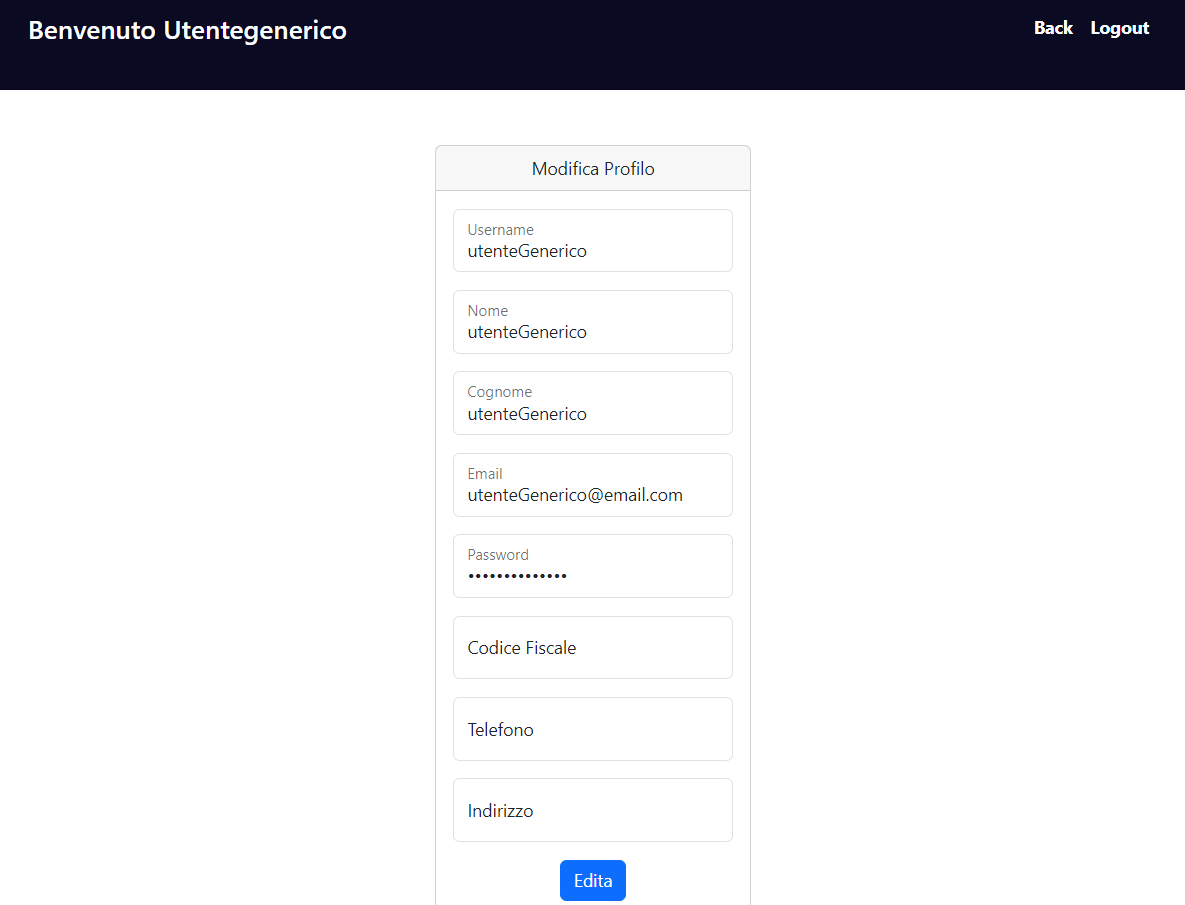
\includegraphics[width=0.95\columnwidth]{utente_generico_modifica.png}}
\end{center}
Cliccando sul tasto "Profilo" ogni utente potrà visualizzare e modificare le informazioni del proprio account.
